\documentclass[xcolor={dvipsnames,table},aspectratio=169]{beamer}
\usepackage[utf8]{inputenc}
\usepackage[T1]{fontenc}
\usepackage[brazil]{babel}
\usepackage{ragged2e}
\usepackage{booktabs}
\usepackage{verbatim}
\usepackage{gensymb}
\usepackage{multirow}
\usepackage{xcolor,colortbl}
\usepackage{tikz}                   
\usetikzlibrary{shadows}
\definecolor{verde}{rgb}{0,0.5,0}
\usepackage{listings}

\lstset{language=C++,
	backgroundcolor=\color{green!10},
	basicstyle=\ttfamily,
	keywordstyle=\color{blue}\ttfamily,
	stringstyle=\color{red}\ttfamily,
	commentstyle=\color{brown}\ttfamily,
	morecomment=[l][\color{magenta}]{\#},
	literate=
	{á}{{\'a}}1
	{à}{{\`a}}1
	{ã}{{\~a}}1
	{â}{{\^a}}1
	{é}{{\'e}}1
	{ê}{{\^e}}1
	{í}{{\'i}}1
	{ó}{{\'o}}1
	{õ}{{\~o}}1
	{ú}{{\'u}}1
	{ü}{{\"u}}1
	{ç}{{\c{c}}}1
	{Á}{{\'A}}1
	{À}{{\`A}}1
	{Ã}{{\~A}}1
	{Â}{{\^A}}1
	{É}{{\'E}}1
	{Ê}{{\^E}}1
	{Í}{{\'I}}1
	{Ó}{{\'O}}1
	{Õ}{{\~O}}1
	{Ú}{{\'U}}1
	{Ü}{{\"U}}1
	{Ç}{{\c{C}}}1
}

\newcommand\setItemnumber[1]{\setcounter{enumi}{\numexpr#1-1\relax}}

\usetheme{AnnArbor}
\usecolortheme{orchid}
\usefonttheme[onlymath]{serif}

\AtBeginSection[]{
  \begin{frame}
  \vfill
  \centering
  \begin{beamercolorbox}[sep=8pt,center,shadow=true,rounded=true]{title}
    \usebeamerfont{title}\insertsectionhead\par%
  \end{beamercolorbox}
  \vfill
  \end{frame}
}

\title[\sc{STL}]{\emph{Standard Template Library} (STL)}
\author[Roland Teodorowitsch]{Roland Teodorowitsch}
%\institute[LP2 - EC - PUCRS]{Laboratório de Programação II - Curso de Engenharia de Computação - PUCRS}
\institute[POO - EC - PUCRS]{Programação Orientada a Objetos - ECo - Curso de Engenharia de Computação - PUCRS}
\date{6 de novembro de 2023}

\begin{document}
\justifying

%-------------------------------------------------------
\begin{frame}
	\titlepage
\end{frame}

%=======================================================
\section{Standard Template Library (STL)}

%-------------------------------------------------------
\begin{frame}\frametitle{\emph{Standard Template Library} (STL)}
\begin{itemize}
	\item Considerando a utilidade do reuso de software e também a utilidade das estruturas de dados e algoritmos utilizados por programadores a \textbf{Standard Template Library (STL)} foi adicionada à biblioteca padrão C++
	\item A \textbf{STL} define componentes genéricos reutilizáveis poderosos que implementam várias estruturas de dados e algoritmos que processam estas estruturas
	\item Basicamente, a \textbf{STL} é composta de \textbf{contêineres}, \textbf{iteradores} e \textbf{algoritmos}
\end{itemize}
\end{frame}

%-------------------------------------------------------
\begin{frame}\frametitle{\emph{Standard Template Library} (STL)}
\begin{itemize}
	\item \textbf{Contêineres} são templates de estruturas de dados
	\begin{itemize}
		\item Possuem métodos associados a eles
	\end{itemize}
	\item \textbf{Iteradores} são semelhantes a ponteiros, utilizados para percorrer e manipular os elementos de um contêiner
	\item \textbf{Algoritmos} são as funções que realizam operações tais como buscar, ordenar e comparar elementos ou contêineres inteiros
	\begin{itemize}
		\item Existem aproximadamente 85 algoritmos implementados na STL
		\item A maioria utiliza iteradores para acessar os elementos de contêineres
	\end{itemize}

\end{itemize}
\end{frame}

%=======================================================
\section{Contêineres}

%-------------------------------------------------------
\begin{frame}\frametitle{Contêineres}
\begin{itemize}
	\item Os contêineres são divididos em três categorias principais
	\begin{enumerate}
		\item \textbf{Contêineres Sequenciais}
		\begin{itemize}
			\item Estruturas de dados lineares
		\end{itemize}
		\item \textbf{Contêineres Associativos}
		\begin{itemize}
			\item Estruturas de dados não lineares
			\item Exploram o conceito de pares chaves/valor
		\end{itemize}
		\item \textbf{Adaptadores de Contêineres}
		\begin{itemize}
			\item São contêineres sequenciais, porém, em versões restringidas
		\end{itemize}
	\end{enumerate}
\end{itemize}
\end{frame}

%-------------------------------------------------------
\begin{frame}\frametitle{Contêineres}
\begin{center}
\begin{tikzpicture}
\node[drop shadow,fill=white,inner sep=0pt] 
{
\rowcolors{1}{RoyalBlue!20}{RoyalBlue!5}
\begin{tabular}{|c|c|p{9cm}|}
\hline
\textbf{Contêineres} & \textbf{Tipo}  & \textbf{Descrição}\\ \hline \hline
\texttt{vector} & Sequencial & Inserções e remoções no final, acesso direto a qualquer elemento.\\ \hline
\texttt{deque}  & Sequencial & Fila duplamente ligada, inserções e remoções no início ou no final, sem acesso direto a qualquer elemento.\\ \hline
\texttt{list}   & Sequencial & Lista duplamente ligada, inserção e remoção em qualquer ponto.\\ \hline\end{tabular}
};
\end{tikzpicture}
\end{center}
\end{frame}

%-------------------------------------------------------
\begin{frame}\frametitle{Contêineres}
\begin{center}
\begin{tikzpicture}
\node[drop shadow,fill=white,inner sep=0pt] 
{
\rowcolors{1}{RoyalBlue!20}{RoyalBlue!5}
\begin{tabular}{|c|c|p{9cm}|}
\hline
\textbf{Contêineres} & \textbf{Tipo}  & \textbf{Descrição}\\ \hline \hline
\texttt{set}     & Associativo & Busca rápida, não permite elementos duplicados.\\ \hline
\texttt{multiset}& Associativo & Busca rápida, permite elementos duplicados.\\ \hline
\texttt{map}     & Associativo & Mapeamento um-para-um, não permite elementos duplicados, busca rápida.\\ \hline
\texttt{multimap}& Associativo & Mapeamento um-para-um, permite elementos duplicados, busca rápida.\\ \hline \hline
\texttt{stack} & Adaptadores & \emph{Last-in, first-out} (LIFO).\\ \hline
\texttt{queue} & Adaptadores & \emph{First-in, first-out} (FIFO).\\ \hline
\texttt{priority\_queue} & Adaptadores & O elemento de maior prioridade é sempre o primeiro elemento a sair.\\ \hline
\end{tabular}
};
\end{tikzpicture}
\end{center}
\end{frame}

%-------------------------------------------------------
\begin{frame}\frametitle{Funções Comuns aos Contêineres}
\begin{itemize}
	\item Todos os contêineres da STL fornecem funcionalidades similares, sendo que muitas operações genéricas se aplicam a todos os contêineres
\end{itemize}
{\small
\begin{center}
\begin{tikzpicture}
\node[drop shadow,fill=white,inner sep=0pt] 
{
\rowcolors{1}{RoyalBlue!20}{RoyalBlue!5}
\begin{tabular}{|c|p{9cm}|}
\hline
\textbf{Funcionalidade}  & \textbf{Descrição}\\ \hline \hline
\texttt{Construtor \emph{default}} & Fornece a inicialização padrão do contêiner.\\ \hline
Construtor Cópia & Construtor que inicializa um contêiner para  ser a cópia de outro do mesmo tipo.\\ \hline
Destrutor & Simplesmente destrói o contêiner quando não for mais necessário.\\ \hline
\texttt{empty} & Retorna \texttt{true} se não houver elementos no contêiner e \texttt{false} caso contrário.\\ \hline
\texttt{size} & Retorna o número de elementos no contêiner.\\ \hline
\texttt{operator=} & Atribui um contêiner a outro.\\ \hline
\texttt{operator<} & Retorna \texttt{true} se o primeiro contêiner for menor que o segundo e \texttt{false} caso contrário.\\ \hline
\end{tabular}
};
\end{tikzpicture}
\end{center}
}
\end{frame}

%-------------------------------------------------------
\begin{frame}\frametitle{Funções Comuns aos Contêineres}
{\small
\begin{center}
\begin{tikzpicture}
\node[drop shadow,fill=white,inner sep=0pt] 
{
\rowcolors{1}{RoyalBlue!20}{RoyalBlue!5}
\begin{tabular}{|c|p{9cm}|}
\hline
\textbf{Funcionalidade}  & \textbf{Descrição}\\ \hline \hline
\texttt{operator<=} & Retorna \texttt{true} se o primeiro contêiner for menor ou igual ao segundo e \texttt{false} caso contrário. \\ \hline
\texttt{operator>} & Retorna \texttt{true} se o primeiro contêiner for maior que o segundo e \texttt{false} caso contrário. \\ \hline
\texttt{operator>=} & Retorna \texttt{true} se o primeiro contêiner for maior ou igual ao segundo e \texttt{false} caso contrário. \\ \hline
\texttt{operator==} & Retorna \texttt{true} se o primeiro contêiner for igual ao segundo e \texttt{false} caso contrário. \\ \hline 
\texttt{operator!=} & Retorna \texttt{true} se o primeiro contêiner for diferente do segundo e \texttt{false} caso contrário. \\ \hline
\texttt{swap} & Troca os elementos de dois contêineres. \\ \hline
\end{tabular}
};
\end{tikzpicture}
\end{center}
}
\begin{itemize}
{\footnotesize
	\item \textbf{Atenção:} Os operadores \texttt{<}, \texttt{<=}, \texttt{>}, \texttt{>=}, \texttt{==} e \texttt{!=} não são fornecidos para o contêiner \texttt{priority\_queue}.
}
\end{itemize}
\end{frame}

%-------------------------------------------------------
\begin{frame}\frametitle{Funções Comuns a Contêineres Sequenciais e Associativos}
{\small
\begin{center}
\begin{tikzpicture}
\node[drop shadow,fill=white,inner sep=0pt] 
{
\rowcolors{1}{RoyalBlue!20}{RoyalBlue!5}
\begin{tabular}{|c|p{9cm}|}
\hline
\textbf{Funcionalidade}  & \textbf{Descrição}\\ \hline \hline
\texttt{max\_size} & Retorna o número máximo de elementos de um contêiner.\\ \hline
\texttt{begin} & As duas versões deste método retornam um \texttt{iterator} ou um \texttt{const\_iterator} para o primeiro elemento do contêiner.\\ \hline
\texttt{end} & As duas versões deste método retornam um \texttt{iterator} ou um \texttt{const\_iterator} para a posição após o final do contêiner.\\ \hline
\texttt{rbegin} &  As duas versões deste método retornam um \texttt{reverse\_iterator} ou um \texttt{const\_reverse\_iterator} para o primeiro elemento do contêiner invertido.\\ \hline
\texttt{rend} &  As duas versões deste método retornam um \texttt{reverse\_iterator} ou um \texttt{const\_reverse\_iterator} para a posição após o final do contêiner invertido.\\ \hline
\texttt{erase} &  Apaga um ou mais elementos do contêiner.\\ \hline
\texttt{clear} &  Apaga todos os elementos do contêiner.\\ \hline
\end{tabular}
};
\end{tikzpicture}
\end{center}
}
\end{frame}

%-------------------------------------------------------
\begin{frame}\frametitle{Arquivos de Cabeçalho da STL}
{\small
\begin{center}
\begin{tikzpicture}
\node[drop shadow,fill=white,inner sep=0pt] 
{
\rowcolors{1}{RoyalBlue!20}{RoyalBlue!5}
\begin{tabular}{|c|p{9cm}|}
\hline
\textbf{Arquivo}  & \textbf{Observação}\\ \hline \hline
\texttt{<vector>} & Vetor\\ \hline
\texttt{<list>} & Lista\\ \hline
\texttt{<deque>} & Fila duplamente ligada\\ \hline
\texttt{<queue>} & Contém \texttt{queue} e \texttt{priority\_queue}\\ \hline
\texttt{<stack>} & Pilha\\ \hline
\texttt{<map>} & Contém \texttt{map} e \texttt{multimap}\\ \hline
\texttt{<set>} & Contém \texttt{set} e \texttt{multiset}\\ \hline
\texttt{<bitset>} & Conjunto de bits (vetor em que cada elemento é um bit -- 0 ou 1)\\ \hline
\end{tabular}
};
\end{tikzpicture}
\end{center}
}
\end{frame}

%-------------------------------------------------------
\begin{frame}\frametitle{Contêineres}
\begin{itemize}
	\item é necessário garantir que os elementos armazenados em um contêiner suportam um conjunto mínimo de operações
	\begin{itemize}
		\item Quando um elemento é inserido em um contêiner, ele é copiado.
		\begin{itemize}
			\item Logo, o operador de atribuição deve ser sobrecarregado se necessário
			\item Também deve haver um construtor cópia
		\end{itemize}
		\item Contêineres associativos e alguns algoritmos requerem que os elementos sejam comparados
		\begin{itemize}
			\item Pelo menos os operadores \texttt{==} e \texttt{<} devem ser sobrecarregados.
		\end{itemize}
	\end{itemize}
\end{itemize}
\end{frame}

%=======================================================
\section{Iteradores}

%-------------------------------------------------------
\begin{frame}\frametitle{Iteradores}
\begin{itemize}
	\item \textbf{Iteradores} são utilizados para apontar elementos de contêineres sequenciais e associativos
	\begin{itemize}
		\item Entre outras coisas
		\item Algumas funcionalidades como \texttt{begin} e \texttt{end} retornam \textbf{iteradores}
		\end{itemize}
	\item Se um \texttt{iterador i} aponta para um elemento:
	\begin{itemize}
		\item \texttt{++i} aponta para o próximo elemento
		\item \texttt{*i} se refere ao conteúdo do elemento apontado por \texttt{i}
		\end{itemize}
\end{itemize}
\end{frame}

%-------------------------------------------------------
\begin{frame}\frametitle{Iteradores}
\begin{itemize}
	\item Os \textbf{iteradores} são objetos declarados no arquivo de cabeçalho \texttt{<iterator>}
	\item Existem basicamente dois tipos de objetos \textbf{iteradores}:
	\begin{itemize}
		\item \texttt{iterator}: aponta para um elemento que pode ser modificado
		\item \texttt{const\_iterator}: aponta para um elemento que não pode ser modificado
		\end{itemize}
	\item Por exemplo, é possível criar \textbf{iteradores} para o \texttt{cin} e o \texttt{cout}
	\begin{itemize}
		\item São sequências de dados, assim como os contêineres
		\item é possível percorrer os dados captados por um \texttt{cin} e os dados a serem escritos por um \texttt{cout}
	\end{itemize}
\end{itemize}
\end{frame}

%-------------------------------------------------------
\begin{frame}[fragile]\frametitle{Iteradores}
\begin{itemize}
	\item Exemplo de iteradores para \texttt{cin} e \texttt{cout}
\begin{lstlisting}[language=C++,basicstyle=\ttfamily\tiny]
#include <iostream>
#include <iterator> // ostream_iterator e istream_iterator

using namespace std;

int main() {
  cout << "Informe dois inteiros: ";
  // cria istream_iterator para ler valores de int a partir de cin
  istream_iterator<int> inputInt(cin);
  int number1 = *inputInt; // le int a partir da entrada padrao
  ++inputInt; // move iterador para o proximo valor de entrada
  int number2 = *inputInt; // le int a partir da entrada padrao
  // cria ostream_iterator para gravar valores int em cout
  ostream_iterator<int> outputInt(cout);
  cout << "A soma eh: ";
  *outputInt = number1 + number2; // gera saida do resultado para cout
  cout << endl;
  return 0;
}
\end{lstlisting}
	\item Saída:
\begin{lstlisting}[language={},basicstyle=\ttfamily\tiny]
Informe dois inteiros: 12 25
A soma eh: 37
\end{lstlisting}
\end{itemize}
\end{frame}

%-------------------------------------------------------
\begin{frame}\frametitle{Categorias de Iteradores}
\begin{columns}
\begin{column}{0.65\linewidth}
{\scriptsize
\begin{center}
\begin{tikzpicture}
\node[drop shadow,fill=white,inner sep=0pt] 
{
\rowcolors{1}{RoyalBlue!20}{RoyalBlue!5}
\begin{tabular}{|c|p{6cm}|}
\hline
\textbf{Categoria}  & \textbf{Descrição}\\ \hline \hline
\emph{input} & Utilizado para ler um elemento de um contêiner. Só se move do início para o final, um elemento por vez. Não pode ser utilizado para percorrer um contêiner mais que uma vez.\\ \hline
\emph{output} & Utilizado para escrever um elemento em um contêiner. Só se move do início para o final, um elemento por vez. Não pode ser utilizado para percorrer um contêiner mais que uma vez.\\ \hline
\emph{forward} & Combina os iteradores \emph{input} e \emph{output} e retém a sua posição no contêiner.\\ \hline
\emph{bidirectional} & Combina o iterador \emph{forward} com a capacidade de se mover do final para o início. Pode ser utilizado para percorrer um contêiner mais que uma vez.\\ \hline
\emph{random access} & Combina o iterador \emph{bidirectional} com a capacidade de acessar diretamente qualquer elemento. Ou seja, pode saltar uma quantidade arbitrária de elementos.\\ \hline
\end{tabular}
};
\end{tikzpicture}
\end{center}
}
\end{column}
\begin{column}{0.35\linewidth}
\begin{figure}[h]
	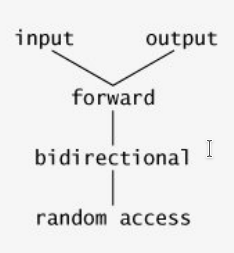
\includegraphics[height=0.25\paperheight]{pucrs-ec-poo-unidade_16-stl-laminas-categorias_de_iteradores.png}
\end{figure}
\begin{itemize}
{\small
	\item Usar o iterador ``mais fraco'' maximiza a reusabilidade.
	\item Por exemplo, um algoritmo que usa um iterador \emph{forward} aceita iteradores \emph{forward}, \emph{bidirectional} ou \emph{random access}.
}
\end{itemize}
\end{column}
\end{columns}
\end{frame}

%-------------------------------------------------------
\begin{frame}\frametitle{Tipos Predefinidos de Iteradores}
{\small
\begin{center}
\begin{tikzpicture}
\node[drop shadow,fill=white,inner sep=0pt] 
{
\rowcolors{1}{RoyalBlue!20}{RoyalBlue!5}
\begin{tabular}{|c|c|c|}
\hline
\textbf{Tipo Predefinido}  & \textbf{Direção do ++} & \textbf{Capacidade}\\ \hline \hline
\texttt{iterator} & Início para o Final & Leitura/Escrita \\ \hline
\texttt{const\_iterator} & Início para o Final & Leitura\\ \hline
\texttt{reverse\_iterator} & Final para o Início & Leitura/Escrita\\ \hline
\texttt{const\_reverse\_iterator} & Final para o Início & Leitura\\ \hline
\end{tabular}
};
\end{tikzpicture}
\end{center}
}
\begin{itemize}
	\item Nem todos os tipos predefinidos o são para todos os contêineres
	\item As versões \textbf\emph{const} são utilizadas para percorrer contêineres de \textbf{somente leitura}
	\item \textbf{Iteradores invertidos} são utilizados para percorrer contêineres na \textbf{direção inversa}
\end{itemize}
\end{frame}

%-------------------------------------------------------
\begin{frame}\frametitle{Operações em Iteradores}
{\small
\begin{center}
\begin{tikzpicture}
\node[drop shadow,fill=white,inner sep=0pt] 
{
\rowcolors{1}{RoyalBlue!20}{RoyalBlue!5}
\begin{tabular}{|c|c|p{8cm}|}
\hline
\textbf{Operação}  & \textbf{Tipo de Iterador} & \textbf{Descrição}\\ \hline \hline
\texttt{++p} & TODOS & Pré-incremento\\ \hline
\texttt{p++} & TODOS & Pós-incremento\\ \hline\hline
\texttt{*p} & \texttt{input} & Referencia o conteúdo apontado\\ \hline
\texttt{p = p1} & \texttt{input} & Atribui um iterador a outro\\ \hline
\texttt{p == p1} & \texttt{input} & Compara dois iteradores quanto à igualdade\\ \hline
\texttt{p != p1} & \texttt{input} & Compara dois iteradores quanto à desigualdade\\ \hline\hline
\texttt{*p} & \texttt{output} & Referencia o conteúdo apontado\\ \hline
\texttt{p = p1} & \texttt{output} & Atribui um iterador a outro\\ \hline
\end{tabular}
};
\end{tikzpicture}
\end{center}
}
\end{frame}

%-------------------------------------------------------
\begin{frame}\frametitle{Operações em Iteradores}
{\small
\begin{center}
\begin{tikzpicture}
\node[drop shadow,fill=white,inner sep=0pt] 
{
\rowcolors{1}{RoyalBlue!20}{RoyalBlue!5}
\begin{tabular}{|c|c|p{8cm}|}
\hline
\textbf{Operação}  & \textbf{Tipo de Iterador} & \textbf{Descrição}\\ \hline \hline
\texttt{p += i} & \texttt{random access} & Incrementa o iterador em \texttt{i} posições\\ \hline
\texttt{p -= i} & \texttt{random access} & Decrementa o iterador em \texttt{i} posições\\ \hline
\texttt{p + i} & \texttt{random access} & Resulta em um iterador posicionado em \texttt{p+i} elementos\\ \hline
\texttt{p - i} & \texttt{random access} & Resulta em um iterador posicionado em \texttt{p-i} elementos\\ \hline
\texttt{p[i]} & \texttt{random access} & Retorna uma referência para o elemento a \texttt{i} posições a partir de \texttt{p}\\ \hline
\texttt{p < p1} & \texttt{random access} & Retonar \texttt{true} se o primeiro iterador estiver antes do segundo no contêiner\\ \hline
\texttt{p <= p1} & \texttt{random access} & Retonar \texttt{true} se o primeiro iterador estiver antes ou na mesma posição do segundo no contêiner\\ \hline
\texttt{p > p1} & \texttt{random access} & Retonar \texttt{true} se o primeiro iterador estiver após o segundo no contêiner\\ \hline
\texttt{p >= p1} & \texttt{random access} & Retonar \texttt{true} se o primeiro iterador estiver após ou na mesma posição do segundo no contêiner\\ \hline
\end{tabular}
};
\end{tikzpicture}
\end{center}
}
\end{frame}

%=======================================================
\section{Algoritmos}

%-------------------------------------------------------
\begin{frame}\frametitle{Algoritmos}
\begin{itemize}
	\item A STL inclui aproximadamente 85 \textbf{algoritmos}
	\begin{itemize}
		\item Podem ser utilizados genericamente, em vários tipos de contêineres
	\end{itemize}
	\item Os \textbf{algoritmos} operam indiretamente sobre os elementos de um contêiner usando iteradores
	\begin{itemize}
		\item Vários deles utilizam pares de iteradores, um apontando para o início e outro apontando para o final
		\item Frequentemente os \textbf{algoritmos} também retornam iteradores como resultado
		\item Este desacoplamento dos contêineres permite que os algoritmos sejam genéricos
	\end{itemize}
	\item A STL é extensível
	\begin{itemize}
		\item Ou seja, é possível adicionar novos algoritmos a ela
	\end{itemize}
\end{itemize}
\end{frame}

%-------------------------------------------------------
\begin{frame}\frametitle{Algoritmos}
\begin{itemize}
	\item Entre os vários algoritmos disponíveis, é possível encontrar:
	\begin{enumerate}
		\item Algoritmos alteradores de sequências:\\
		\texttt{copy}, \texttt{remove}, \texttt{reverse\_copy}, \texttt{copy\_backward}, \texttt{remove\_copy}, \texttt{rotate}, \texttt{fill}, \texttt{remove\_copy\_if}, \texttt{rotate\_copy}, \texttt{fill\_n}, \texttt{remove\_if}, \texttt{stable\_partition}, \texttt{generate}, \texttt{replace}, \texttt{swap}, \texttt{generate\_n}, \texttt{replace\_copy}, \texttt{swap\_ranges}, \texttt{iter\_swap}, \texttt{replace\_copy\_if}, \texttt{transform}, \texttt{partition}, \texttt{replace\_if}, \texttt{unique}, \texttt{random\_shuffle}, \texttt{reverse}, \texttt{unique\_copy}
		\item Algoritmos não alteradores de sequências:\\
		\texttt{adjacent\_find}, \texttt{find}, \texttt{find\_if}, \texttt{count}, \texttt{find\_each}, \texttt{mismatch}, \texttt{count\_if}, \texttt{find\_end}, \texttt{search}, \texttt{equal}, \texttt{find\_first\_of}, \texttt{search\_n}
		\item Algoritmos numéricos (definidos em \texttt{<numeric>}):\\
		\texttt{accumulate}, \texttt{partial\_sum}, \texttt{inner\_product}, \texttt{adjacent\_difference}
	\end{enumerate}

\end{itemize}
\end{frame}

%-------------------------------------------------------
\begin{frame}\frametitle{Exemplos de Algoritmos}
\begin{itemize}
	\item Ordenação:
{\footnotesize
\begin{center}
\begin{tikzpicture}
\node[drop shadow,fill=white,inner sep=0pt] 
{
\rowcolors{1}{RoyalBlue!20}{RoyalBlue!5}
\begin{tabular}{|c|p{10cm}|}
\hline
\textbf{Algoritmo}  & \textbf{Descrição}\\ \hline \hline
\texttt{sort} & Ordena os elementos do contêiner\\ \hline
\texttt{stable\_sort} & Ordena os elementos do contêiner preservando a ordem relativa dos equivalentes\\ \hline
\texttt{partial\_sort} & Ordena parcialmente o contêiner\\ \hline
\texttt{partial\_sort\_copy} & Copia os menores elementos e os ordena no contêiner de destino\\ \hline
\texttt{nth\_element} & Ordena o n-ésimo elemento\\ \hline
\end{tabular}
};
\end{tikzpicture}
\end{center}
}
	\item Busca Binária:
{\footnotesize
\begin{center}
\begin{tikzpicture}
\node[drop shadow,fill=white,inner sep=0pt] 
{
\rowcolors{1}{RoyalBlue!20}{RoyalBlue!5}
\begin{tabular}{|c|p{10cm}|}
\hline
\texttt{lower\_bound} & Retorna um iterador para o limite esquerdo\\ \hline
\texttt{upper\_bound} & Retorna um iterador para o limite direito\\ \hline
\texttt{equal\_range} & Retorna os limites que incluem um conjunto de elementos com um determinado valor\\ \hline
\texttt{binary\_search} & Testa se um valor existe em um intervalo\\ \hline
\end{tabular}
};
\end{tikzpicture}
\end{center}
}
\end{itemize}
\end{frame}

%-------------------------------------------------------
\begin{frame}\frametitle{Exemplos de Algoritmos}
\begin{itemize}
	\item Intercalação:
{\footnotesize
\begin{center}
\begin{tikzpicture}
\node[drop shadow,fill=white,inner sep=0pt] 
{
\rowcolors{1}{RoyalBlue!20}{RoyalBlue!5}
\begin{tabular}{|c|p{9cm}|}
\hline
\textbf{Algoritmo}  & \textbf{Descrição}\\ \hline \hline
\texttt{merge} & Intercala os elementos de dois intervalos e coloca o resultado em outro intervalo\\ \hline
\texttt{inplace\_merge} & Intercala os elementos de dois intervalos e coloca o resultado no mesmo intervalo\\ \hline
\texttt{includes} & Testa se um intervalo ordenado inclui outro intervalo ordenado, se cada elemento de um intervalo é equivalente a outro do segundo intervalo\\ \hline
\texttt{set\_union} & Calcula a união entre dois intervalos de valores\\ \hline
\texttt{set\_intersection} & Calcula a interseção entre dois intervalos de valores\\ \hline
\texttt{set\_difference} & Calcula a diferença entre dois intervalos de valores\\ \hline
\texttt{set\_symmetric\_difference} & Calcula a diferença simétrica entre dois intervalos de valores\\ \hline
\end{tabular}
};
\end{tikzpicture}
\end{center}
}
\end{itemize}
\end{frame}

%-------------------------------------------------------
\begin{frame}\frametitle{Exemplos de Algoritmos}
\begin{itemize}
	\item \emph{Heap}:
{\footnotesize
\begin{center}
\begin{tikzpicture}
\node[drop shadow,fill=white,inner sep=0pt] 
{
\rowcolors{1}{RoyalBlue!20}{RoyalBlue!5}
\begin{tabular}{|c|p{9cm}|}
\hline
\textbf{Algoritmo}  & \textbf{Descrição}\\ \hline \hline
\texttt{push\_heap} & Adiciona um elemento a um \emph{heap}\\ \hline
\texttt{pop\_heap} & Remove um elemento de um \emph{heap}\\ \hline
\texttt{make\_heap} & Cria um \emph{heap} a partir de um intervalo de valores\\ \hline
\texttt{sort\_heap} & Ordena os elementos de um \emph{heap}\\ \hline
\end{tabular}
};
\end{tikzpicture}
\end{center}
}
\end{itemize}
\end{frame}

%-------------------------------------------------------
\begin{frame}\frametitle{Exemplos de Algoritmos}
\begin{itemize}
	\item Min/Max:
{\footnotesize
\begin{center}
\begin{tikzpicture}
\node[drop shadow,fill=white,inner sep=0pt] 
{
\rowcolors{1}{RoyalBlue!20}{RoyalBlue!5}
\begin{tabular}{|c|p{9cm}|}
\hline
\textbf{Algoritmo}  & \textbf{Descrição}\\ \hline \hline
\texttt{min} & Retorna o menor de dois argumentos\\ \hline
\texttt{max} & Retorna o maior de dois argumentos\\ \hline
\texttt{min\_element} & Retorna o menor elemento de uma sequência\\ \hline
\texttt{max\_element} & Retorna o maior elemento de uma sequência\\ \hline
\texttt{lexicographical\_compare} & Comparação lexicográfica (menor que)\\ \hline
\texttt{next\_permutation} & Transforma uma sequência na próxima permutação (ordem lexicográfica)\\ \hline
\texttt{prev\_permutation} & Transforma uma sequência na permutação anterior (ordem lexicográfica)\\ \hline
\end{tabular}
};
\end{tikzpicture}
\end{center}
}
\end{itemize}
\end{frame}

%=======================================================
\section{Exemplos Completos}

%-------------------------------------------------------
\begin{frame}\frametitle{\texttt{vector}}
\begin{itemize}
	\item A classe \textbf{\texttt{vector}} é genérica, logo, deve-se definir o tipo na declaração de um objeto
	\item Este contêiner é dinâmico
	\begin{itemize}
		\item A cada inserção o contêiner se redimensiona automaticamente
	\end{itemize}
	\item O método \texttt{push\_back} adiciona um elemento ao final do \texttt{vector}
	\item Outros possíveis métodos incluem:
	\begin{itemize}
		\item \texttt{front}: determina o primeiro elemento
		\item \texttt{back}: determina o último elemento
		\item \texttt{at}: determina o elemento em uma determinada posição, mas antes verifica se é uma posição válida
		\item \texttt{insert}: insere um elemento em uma posição especificada por um iterador
	\end{itemize}
\end{itemize}
\end{frame}

%-------------------------------------------------------
\begin{frame}[fragile]\frametitle{\texttt{vector}: exemplo 1}
\begin{columns}
\begin{column}{0.5\linewidth}
\begin{lstlisting}[language=C++,basicstyle=\ttfamily\tiny]
#include <iostream>
#include <vector>
using namespace std;
int main () {
  vector<int> v1;   // vetor vazio de inteiros
  cout << "v1.size()=" << v1.size() << endl;
  for ( vector<int>::iterator it = v1.begin();
        it != v1.end(); ++it)
      cout << ' ' << *it;
  cout << '\n';

  vector<int> v2 (4,100);   // quatro ints com 100
  cout << "v2.size()=" << v2.size() << endl;
  for ( vector<int>::iterator it = v2.begin();
        it != v2.end(); ++it)
      cout << ' ' << *it;
  cout << '\n';

  vector<int> v3 (v2.begin(),v2.end()); // it. de v2
  cout << "v3.size()=" << v3.size() << endl;
  for ( vector<int>::iterator it = v3.begin();
        it != v3.end(); ++it)
      cout << ' ' << *it;
  cout << '\n';
\end{lstlisting}
\end{column}
\begin{column}{0.5\linewidth}
\begin{lstlisting}[language=C++,basicstyle=\ttfamily\tiny]
  vector<int> v4 (v3);  // uma copia de v3
  cout << "v4.size()=" << v4.size() << endl;
  for (vector<int>::iterator it = v4.begin();
     it != v4.end(); ++it)
    cout << ' ' << *it;
  cout << '\n';

  // o construtor tambem pode ser usado com arrays
  int myints[] = {16,2,77,29};
  vector<int> v5 (myints, myints + sizeof(myints) / sizeof(int) );
  cout << "O conteudo de v5 eh:";
  for ( vector<int>::iterator it = v5.begin();
        it != v5.end(); ++it)
      cout << ' ' << *it;
  cout << '\n';
  cout << *v5.begin() << endl;
  cout << v5.begin()[0] << endl;
  cout << v5[0] << endl;
  cout << *(v5.end()-1) << endl;
  cout << v5[v5.size()-1] << endl;

  return 0;
}
\end{lstlisting}
\end{column}
\end{columns}
\end{frame}

%-------------------------------------------------------
\begin{frame}[fragile]\frametitle{\texttt{vector}: exemplo 2}
\begin{lstlisting}[language=C++,basicstyle=\ttfamily\tiny]
#include <iostream>
#include <vector>
using namespace std;
int main() {
  vector<int>::const_iterator it;
  vector <int> v1;
  cout << "v1.size()=" << v1.size() << endl;
  cout << "v1.max_size()=" << v1.max_size() << endl;
  if (v1.empty())
     cout << "vazio...";
  else
     for (it=v1.begin(); it!=v1.end(); ++it)
         cout << *it << ' ';
  cout << endl;
  cout << "v1.push_back(12);" << endl;
  v1.push_back(12);
  cout << "v1.push_back(34);" << endl;
  v1.push_back(34);
  cout << "v1.push_back(56);" << endl;
  v1.push_back(56);
  cout << "v1.size()=" << v1.size() << endl;
  for (it=v1.begin(); it!=v1.end(); ++it)
      cout << *it << ' ';
  cout << endl;
  return 0;
}
\end{lstlisting}
\end{frame}

%-------------------------------------------------------
\begin{frame}[fragile]\frametitle{\texttt{vector}: exemplo 3}
\begin{columns}
\begin{column}{0.46\linewidth}
\begin{lstlisting}[language=C++,basicstyle=\ttfamily\tiny]
#include <iostream>
#include <vector>
using namespace std;
int main() {
  vector<int>::const_iterator it;
  vector<int>::iterator it2;
  vector <int> v2(10);
  cout << "v2.size()=" << v2.size() << endl;
  cout << "v2.max_size()=" << v2.max_size() << endl;
  if (v2.empty()) cout << "vazio..." << endl;
  else {
     for (it=v2.begin(); it!=v2.end(); ++it)
         cout << *it << ' ';
     cout << endl;
     int x = 10;
     for (it2=v2.begin(); it2!=v2.end(); ++it2) {
         *it2 = x;
         x += 10;
     }
     for (it=v2.begin(); it!=v2.end(); ++it)
         cout << *it << ' ';
     cout << endl;
     v2.pop_back();
     v2.pop_back();
     cout << "2 x v2.pop_back();" << endl;
     cout << "v2.size()=" << v2.size() << endl;
\end{lstlisting}
\end{column}
\begin{column}{0.54\linewidth}
\begin{lstlisting}[language=C++,basicstyle=\ttfamily\tiny]
     for (it=v2.begin(); it!=v2.end(); ++it)
         cout << *it << ' ';
     cout << endl;
     v2.erase(v2.begin()+1);
     cout << "v2.erase(v2.begin()+1);" << endl;
     cout << "v2.size()=" << v2.size() << endl;
     for (it=v2.begin(); it!=v2.end(); ++it)
         cout << *it << ' ';
     cout << endl;
     // Apaga elementos de ind. 4 (5.) ate ind. 5 (6.)
     v2.erase(v2.begin()+4,v2.begin()+6);
     cout << "v2.erase(v2.begin()+4,v2.begin()+6);" << endl;
     cout << "v2.size()=" << v2.size() << endl;
     for (it=v2.begin(); it!=v2.end(); ++it)
         cout << *it << ' ';
     cout << endl;
     it=v2.begin();
     for (int i=0; i<v2.size(); ++i) cout << *(it+i) << ' ';
     cout << endl;
     for (int i=0; i<v2.size(); ++i) cout << it[i] << ' ';
     cout << endl;
     for (int i=0; i<v2.size(); ++i) cout << v2[i] << ' ';
     cout << endl;
  }
  return 0;
}
\end{lstlisting}
\end{column}
\end{columns}
\end{frame}

%-------------------------------------------------------
\begin{frame}\frametitle{\texttt{list}}
\begin{itemize}
	\item No exemplo a seguir, os seguintes métodos da classe list são usados:
	\begin{itemize}
		\item \texttt{sort}: ordena a lista em ordem crescente
		\item \texttt{unique}: remove elementos duplicados
		\item \texttt{remove}: apaga todas as ocorrências de um determinado valor da lista
	\end{itemize}
	\item Existem outros como:
	\begin{itemize}
		\item \texttt{reverse}: inverte a lista
		\item \texttt{merge}: intercala listas
		\item \texttt{remove\_if}: remove elementos que atendam um critério
	\end{itemize}
\end{itemize}
\end{frame}

%-------------------------------------------------------
\begin{frame}[fragile]\frametitle{\texttt{list}: exemplo 1}
\begin{columns}
\begin{column}{0.5\linewidth}
\begin{lstlisting}[language=C++,basicstyle=\ttfamily\tiny]
#include <iostream>
#include <list>
using namespace std;
void mostraLista(string nome,list<int> l) {
  cout << nome << " = { ";
  list<int>::iterator it;
  for (it = l.begin(); it != l.end(); it++) {
      if (it != l.begin()) cout << ',';
      cout << *it;
  }
  cout << " }" << endl;
}
int main () {
  // lista de 4 inteiros com valor 100
  list<int> first (4,100);
  mostraLista("first", first);
  // lista criada a partir de outra
  list<int> second (first.begin(),first.end());
  mostraLista("second", second);
  // lista criada com construtor de copia
  list<int> third (second);
  mostraLista("third", third);
  // a lista pode ser criada a partir de um array
  int v[] = { 2, 3, 5, 7, 11};
  list<int> fourth (v, v + sizeof(v)/sizeof(int) );
  mostraLista("fourth", fourth);
\end{lstlisting}
\end{column}
\begin{column}{0.5\linewidth}
\begin{lstlisting}[language=C++,basicstyle=\ttfamily\tiny]
  list<int> fifth;       // lista de inteiros vazia
  mostraLista("fifth", fifth);
  fifth.push_front( 1 ); //insere na frente
  mostraLista("fifth", fifth);
  fifth.push_front( 2 );
  mostraLista("fifth", fifth);
  fifth.push_front( 3 );
  mostraLista("fifth", fifth);
  fifth.push_back( 4 );  //insere no final
  mostraLista("fifth", fifth);
  fifth.push_back( 1 );
  mostraLista("fifth", fifth);
  fifth.sort();          // ordena a lista
  mostraLista("fifth", fifth);
  fifth.remove( 4 );     // remove todos os 4s
  mostraLista("fifth", fifth);
  fifth.unique();        // remove elementos duplicados
  mostraLista("fifth", fifth);
  fifth.pop_front();     // remove elemento do inicio
  mostraLista("fifth", fifth);
  fifth.pop_back();      // remove elemento do fim
  mostraLista("fifth", fifth);
  fifth.clear();         // esvazia a lista
  mostraLista("fifth", fifth);
  return 0;
}
\end{lstlisting}
\end{column}
\end{columns}
\end{frame}

%-------------------------------------------------------
\begin{frame}\frametitle{\texttt{deque}}
\begin{itemize}
	\item Não possui, por exemplo, os métodos \texttt{sort()}, \texttt{remove()} e \texttt{unique()}
	\item O método \texttt{push\_front()} está disponível apenas para \texttt{list} e \texttt{deque}
	\item O operador \texttt{[]} permite acesso direto aos elementos do \texttt{deque}
	\begin{itemize}
		\item Também pode ser utilizado em um \texttt{vector}
	\end{itemize}
	\item Em geral, um \texttt{deque} possui um desempenho levemente inferior em relação a um \texttt{vector}
	\begin{itemize}
		\item No entanto, é mais eficiente para fazer inserções e remoções no início
	\end{itemize}
\end{itemize}
\end{frame}

%-------------------------------------------------------
\begin{frame}[fragile]\frametitle{\texttt{deque}: exemplo 1}
\begin{columns}
\begin{column}{0.5\linewidth}
\begin{lstlisting}[language=C++,basicstyle=\ttfamily\tiny]
#include <iostream>
#include <deque>

using namespace std;

void mostraDeque(string nome,deque<int> l) {
  cout << nome << " = { ";
  deque<int>::iterator it;
  for (it = l.begin(); it != l.end(); it++) {
      if (it != l.begin()) cout << ',';
      cout << *it;
  }
  cout << " }" << endl;
}

int main () {
  // deque de 4 inteiros com valor 100
  deque<int> first (4,100);
  mostraDeque("first", first);
  // deque criado a partir de outro
  deque<int> second (first.begin(),first.end());
  mostraDeque("second", second);
  // deque criado com construtor de copia
  deque<int> third (second);
  mostraDeque("third", third);
\end{lstlisting}
\end{column}
\begin{column}{0.5\linewidth}
\begin{lstlisting}[language=C++,basicstyle=\ttfamily\tiny]
  // o deque pode ser criado a partir de um array
  int v[] = { 2, 3, 5, 7, 11};
  deque<int> fourth (v, v + sizeof(v)/sizeof(int) );
  mostraDeque("fourth", fourth);
  // deque de inteiros vazio
  deque<int> fifth;
  mostraDeque("fifth", fifth);
  fifth.push_front( 1 ); //insere na frente
  mostraDeque("fifth", fifth);
  fifth.push_front( 2 );
  mostraDeque("fifth", fifth);
  fifth.push_front( 3 );
  mostraDeque("fifth", fifth);
  fifth.push_back( 4 );  //insere no final
  mostraDeque("fifth", fifth);
  fifth.push_back( 1 );
  mostraDeque("fifth", fifth);
  fifth.pop_front();     // remove elemento do inicio
  mostraDeque("fifth", fifth);
  fifth.pop_back();      // remove elemento do fim
  mostraDeque("fifth", fifth);
  fifth.clear();         // esvazia o Deque
  mostraDeque("fifth", fifth);
  return 0;
}
\end{lstlisting}
\end{column}
\end{columns}
\end{frame}

%=======================================================
\section{Lista de Exercícios}

%-------------------------------------------------------
\begin{frame}[fragile]\frametitle{Exercício 1}
\begin{enumerate}
	\setItemnumber{1}
	\item Considere a definição da classe \texttt{Turma} abaixo.
\lstinputlisting[basicstyle=\ttfamily\tiny]{src/Turma.hpp}
\end{enumerate}
\end{frame}

%-------------------------------------------------------
\begin{frame}[fragile]\frametitle{Exercício 1}
\begin{enumerate}
	\setItemnumber{1}
	\item (Continuação)\\
	Implemente a classe \texttt{Turma} em um arquivo \texttt{Turma.cpp} e também uma aplicação que crie uma lista (usando o contêiner \texttt{list} da STL) com no mínimo 5 turmas. Nessa aplicação, depois de adicionar as turmas na lista e de mostrar a lista, utilize o método \texttt{sort()} do contêiner \texttt{list} para ordenar a lista. Por fim, mostre a lista ordenada.\\
O método \texttt{void adicionaEncontro(int ds, string h)} recebe um dia da semana e um horário, adicionando ambos com \texttt{push\_back()}, respectivamente, nas variáveis de instância 
\texttt{vector<int> diaSemana} e \texttt{vector<string> horario}.\\
Observe que a ordenação padrão necessita e utiliza os métodos sobrecarregados para os operadores ``=='' e ``<'' (estes métodos devem utilizar como critério de ordenação apenas o código da turma).
\end{enumerate}
\end{frame}

%-------------------------------------------------------
\begin{frame}[fragile]\frametitle{Exercício 2}
\begin{enumerate}
	\setItemnumber{2}
	\item Usando as implementações da classe \texttt{Turma} do Exercício 1, \texttt{Turma.hpp} e \texttt{Turma.cpp}, altere a aplicação para usar \texttt{vector} no lugar de \texttt{list}.\\
Será necessário fazer alterações na estratégia de ordenação, pois o contêiner \texttt{vector} NÃO possui o método \texttt{sort()}, sendo necessário usar a função \texttt{sort()} declarada no arquivo de cabeçalho \texttt{algorithm}.\\
Além de mostrar a lista ordenada pelo critério padrão (ou seja pelo código), mostre a lista ordenada usando o seguinte conjunto de critérios: nome (primeiro critério), código (segundo critério -- será usado quando os nomes forem iguais) e turma (terceiro critério -- será usado quando nomes e códigos forem iguais). Para isto implemente a comparação entre turmas em uma função \texttt{bool compTurma(Turma \&t1, Turma \&t2)}.
\end{enumerate}
\end{frame}

%-------------------------------------------------------
\begin{frame}[fragile]\frametitle{Exercícios 3, 4 e 5}
\begin{enumerate}
	\setItemnumber{3}
	\item Escreva um programa usando o contêiner \texttt{vector} da STL que declara um vetor de inteiros. Leia valores inteiros do terminal, enquanto eles NÃO forem negativos, armazenando os valores lidos no vetor. Por fim, imprima o vetor de inteiros na saída padrão.
	\item Escreva um programa que explora STL, o qual captura uma sequência arbitrária de dígitos binários com \texttt{cin} e armazena em um contêiner. Enquanto o valor recebido é diferente de 1 ou 0. Considere que o primeiro valor inserido é o \emph{bit} menos significativos. Ao final, apresente a representação binária informada e o valor decimal sem sinal desta representação binária.
	\item Implemente um programa que lê \texttt{n} palavras da entrada-padrão, e mais uma palavra-chave. Você deve localizar e imprimir as palavras que foram digitadas que possuem a palavra-chave como substring.\\
	\textbf{Dica:} use o método \texttt{find()} da classe \texttt{string}. Este método retorna \texttt{string::npos} se não encontrar nada.
\end{enumerate}
\end{frame}


%-------------------------------------------------------
\begin{frame}[fragile]\frametitle{Exercício 6}
\begin{enumerate}
	\setItemnumber{6}
	\item Escreva um programa que recebe de entrada nomes e telefones correspondentes.
	\begin{enumerate}[a]
		\item A entrada deve ser \texttt{n} nomes e \texttt{n} telefones. Defina uma classe e seus métodos para armazenamento de tais informações.
		\item Na saída, imprima a lista \texttt{[<nome> <telefone>]} ordenada pelos nomes. Crie uma função para comparação. Explore o algoritmo sort de STL. Veja exemplo em: \url{http://www.inf.pucrs.br/~pinho/PRGSWB/STL/stl.html}.
		\item Após isso, o programa deve ler um nome da entrada padrão e imprimir seu telefone correspondente, se este existir. Se não existir, imprima uma mensagem apropriada.
	\end{enumerate}
\end{enumerate}
\end{frame}

%-------------------------------------------------------
\begin{frame}[fragile]\frametitle{Exercício 7}
\begin{enumerate}
	\setItemnumber{7}
	\item Uma pilha (\emph{stack}) é um tipo abstrato de dados que tem associadas as seguintes operações:\\
	\begin{itemize}
		\item \texttt{push()} -- coloca um novo elemento no topo da pilha
		\item \texttt{pop()} -- retira um elemento do topo da pilha
		\item \texttt{top()} -- devolve o elemento no topo da pilha (sem a alterar!)
		\item \texttt{clear()} -- esvazia a pilha
	\end{itemize}
	Defina:\\
	\begin{itemize}
		\item Uma classe genérica em C++ que implemente uma pilha com todas as operações mencionadas e utiliza como estrutura de armazenamento um \emph{array}. (Sugestão: utilize a classe \texttt{vector} da STL.)
		\item Uma classe genérica em C++ que implementa uma pilha com todas as operações mencionadas e utiliza como estrutura de armazenamento uma lista ligada. (Sugestão: utilize a classe \texttt{list} da STL.)
	\end{itemize}
\end{enumerate}
\end{frame}

%-------------------------------------------------------
\begin{frame}[fragile]\frametitle{Exercício 8}
\begin{enumerate}
	\setItemnumber{8}
	\item Considere um sistema de impressão que utiliza duas políticas de atendimento dos trabalhos de impressão:\\
	\begin{itemize}
		\item P1 -- imprime pela ordem de chegada;
		\item P2 -- imprime o menor trabalho primeiro.
	\end{itemize}
Assuma que o tempo de impressão por página é uma constante e que o número máximo de páginas é 50.\\
	\begin{itemize}
		\item Gere 10 sessões de impressão e meça o tempo médio que um utilizador espera pelo seu trabalho se utilizar a política P1 em cada sessão. Para cada sessão de impressão gere aleatoriamente T trabalhos, cada um com um número de páginas também aleatório. Para o armazenamento dos trabalhos, utilize a classe queue da STL.
		\item Repita o item anterior utilizando, agora, a política P2.
		\item Identifique a melhor política, no sentido em que minimiza o tempo médio de espera dos utilizadores.
	\end{itemize}
\end{enumerate}
\end{frame}

%=======================================================
\section{Fontes de consulta}

%-------------------------------------------------------
\begin{frame}\frametitle{Fontes de consulta}
\begin{itemize}
	\item Geral: \url{http://en.cppreference.com/w/cpp/container}
	\item \texttt{vector}: \url{http://en.cppreference.com/w/cpp/container/vector}
	\item \texttt{list}: \url{http://en.cppreference.com/w/cpp/container/list}
\end{itemize}
\end{frame}

%=======================================================
\section{Creditos}

%-------------------------------------------------------
\begin{frame}\frametitle{Creditos}
\begin{itemize}
	\item Estas lâminas contêm trechos de materiais disponibilizados pelos professores Rafael Garibotti e Edson Moreno.
\end{itemize}
\end{frame}

%=======================================================
\section{Soluções}

%-------------------------------------------------------
\begin{frame}[fragile]\frametitle{Exercício 1: \texttt{Turma.cpp}}
\lstinputlisting[basicstyle=\ttfamily\tiny]{src/Turma.cpp}
\end{frame}

%-------------------------------------------------------
\begin{frame}[fragile]\frametitle{Exercício 1: \texttt{exercicio1.cpp}}
\fontsize{3pt}{5pt}\selectfont{
\lstinputlisting[]{src/exercicio1.cpp}
}
\end{frame}

%-------------------------------------------------------
\begin{frame}[fragile]\frametitle{Exercício 2: \texttt{exercicio2.cpp}}
\fontsize{3pt}{5pt}\selectfont{
\lstinputlisting[]{src/exercicio2.cpp}
}
\end{frame}

%-------------------------------------------------------
\begin{frame}[fragile]\frametitle{Exercício 3: \texttt{exercicio3.cpp}}
\lstinputlisting[basicstyle=\ttfamily\tiny]{src/exercicio3.cpp}
\end{frame}

%-------------------------------------------------------
\end{document}
